\documentclass{standalone}
%
\usepackage{tikz}
\usetikzlibrary{backgrounds,bending,arrows.meta,shapes.callouts}
%
\usepackage{tkz-euclide}
\usetkzobj{all}
%
\usepackage{xcolor}
\definecolor{space}{HTML}{0A2543}
\definecolor{earth}{HTML}{0089FA}
\definecolor{dida}{HTML}{FFDE00}
\definecolor{title}{HTML}{FBA706}
\definecolor{moon}{HTML}{AFAFAF}
\definecolor{craterm}{HTML}{616060}
%
\usepackage{amsmath}
%
\usepackage{fontspec}
\setmainfont{Open Dyslexic}
%
\title{Flyby Bepi-Colombo}
\begin{document}
	\tikzset{notice/.style  = { draw, ellipse callout, callout relative pointer={#1} },
		human/.pic = {
			\draw [fill] (0,0) circle (0.3cm);
			\draw [thick] (0,0) circle -- (0,-1.5);
			\draw [thick] (-0.5,-1) -- (0,-0.5) -- (0.5,-1);
			\draw [thick] (-0.5,-2) -- (0,-1.5) -- (0.5,-2);
		},
	}
	\begin{tikzpicture}[background rectangle/.style={fill=white},show background rectangle,>={[inset=0,angle'=27]Stealth}]
		%title
		\draw [black,ultra thick,fill=title] (0,7) rectangle (30,15);
		\node (example-textwidth-2) [right, align=center, text width=30cm, color=black, font=\fontsize{90pt}{91pt}\selectfont] at (0,11) {L'eclissi di Sole};
		%sun-moon-earth comic
		\begin{scope}[shift={(0,0)}]
			\draw [ultra thick, fill=space] (1.5,6) rectangle (28.5,-14);
			\node at (7,0) {
\includegraphics[width=12cm]{sun}};
			\node at (15,-5) {
\includegraphics[width=4cm]{moon}};
			\node at (23,-10) {
\includegraphics[width=7cm]{earth}};
			\node (example-textwidth-2) [notice={(3.5,2)}, ultra thick, right, align=center, text width=7cm, color=black, fill=white, font=\fontsize{23pt}{24pt}\selectfont] at (3,-10) {Guarda! Ora ti passo davanti! Bll... Bll...};
			\node (example-textwidth-2) [notice={(-3,-0.5)}, ultra thick, right, align=center, text width=7cm, color=black, fill=white, font=\fontsize{23pt}{24pt}\selectfont] at (15,1) {Ringrazia che siete lontane...};
			\node (example-textwidth-2) [notice={(-0.5,-1)}, ultra thick, right, align=center, text width=3cm,, color=black, fill=white, font=\fontsize{16pt}{17pt}\selectfont] at (23,-5) {Oh! Holy Moon...};
		\end{scope}
		%tolomeo
		\begin{scope}[shift={(0,-19)}]
			\node at (5,0) {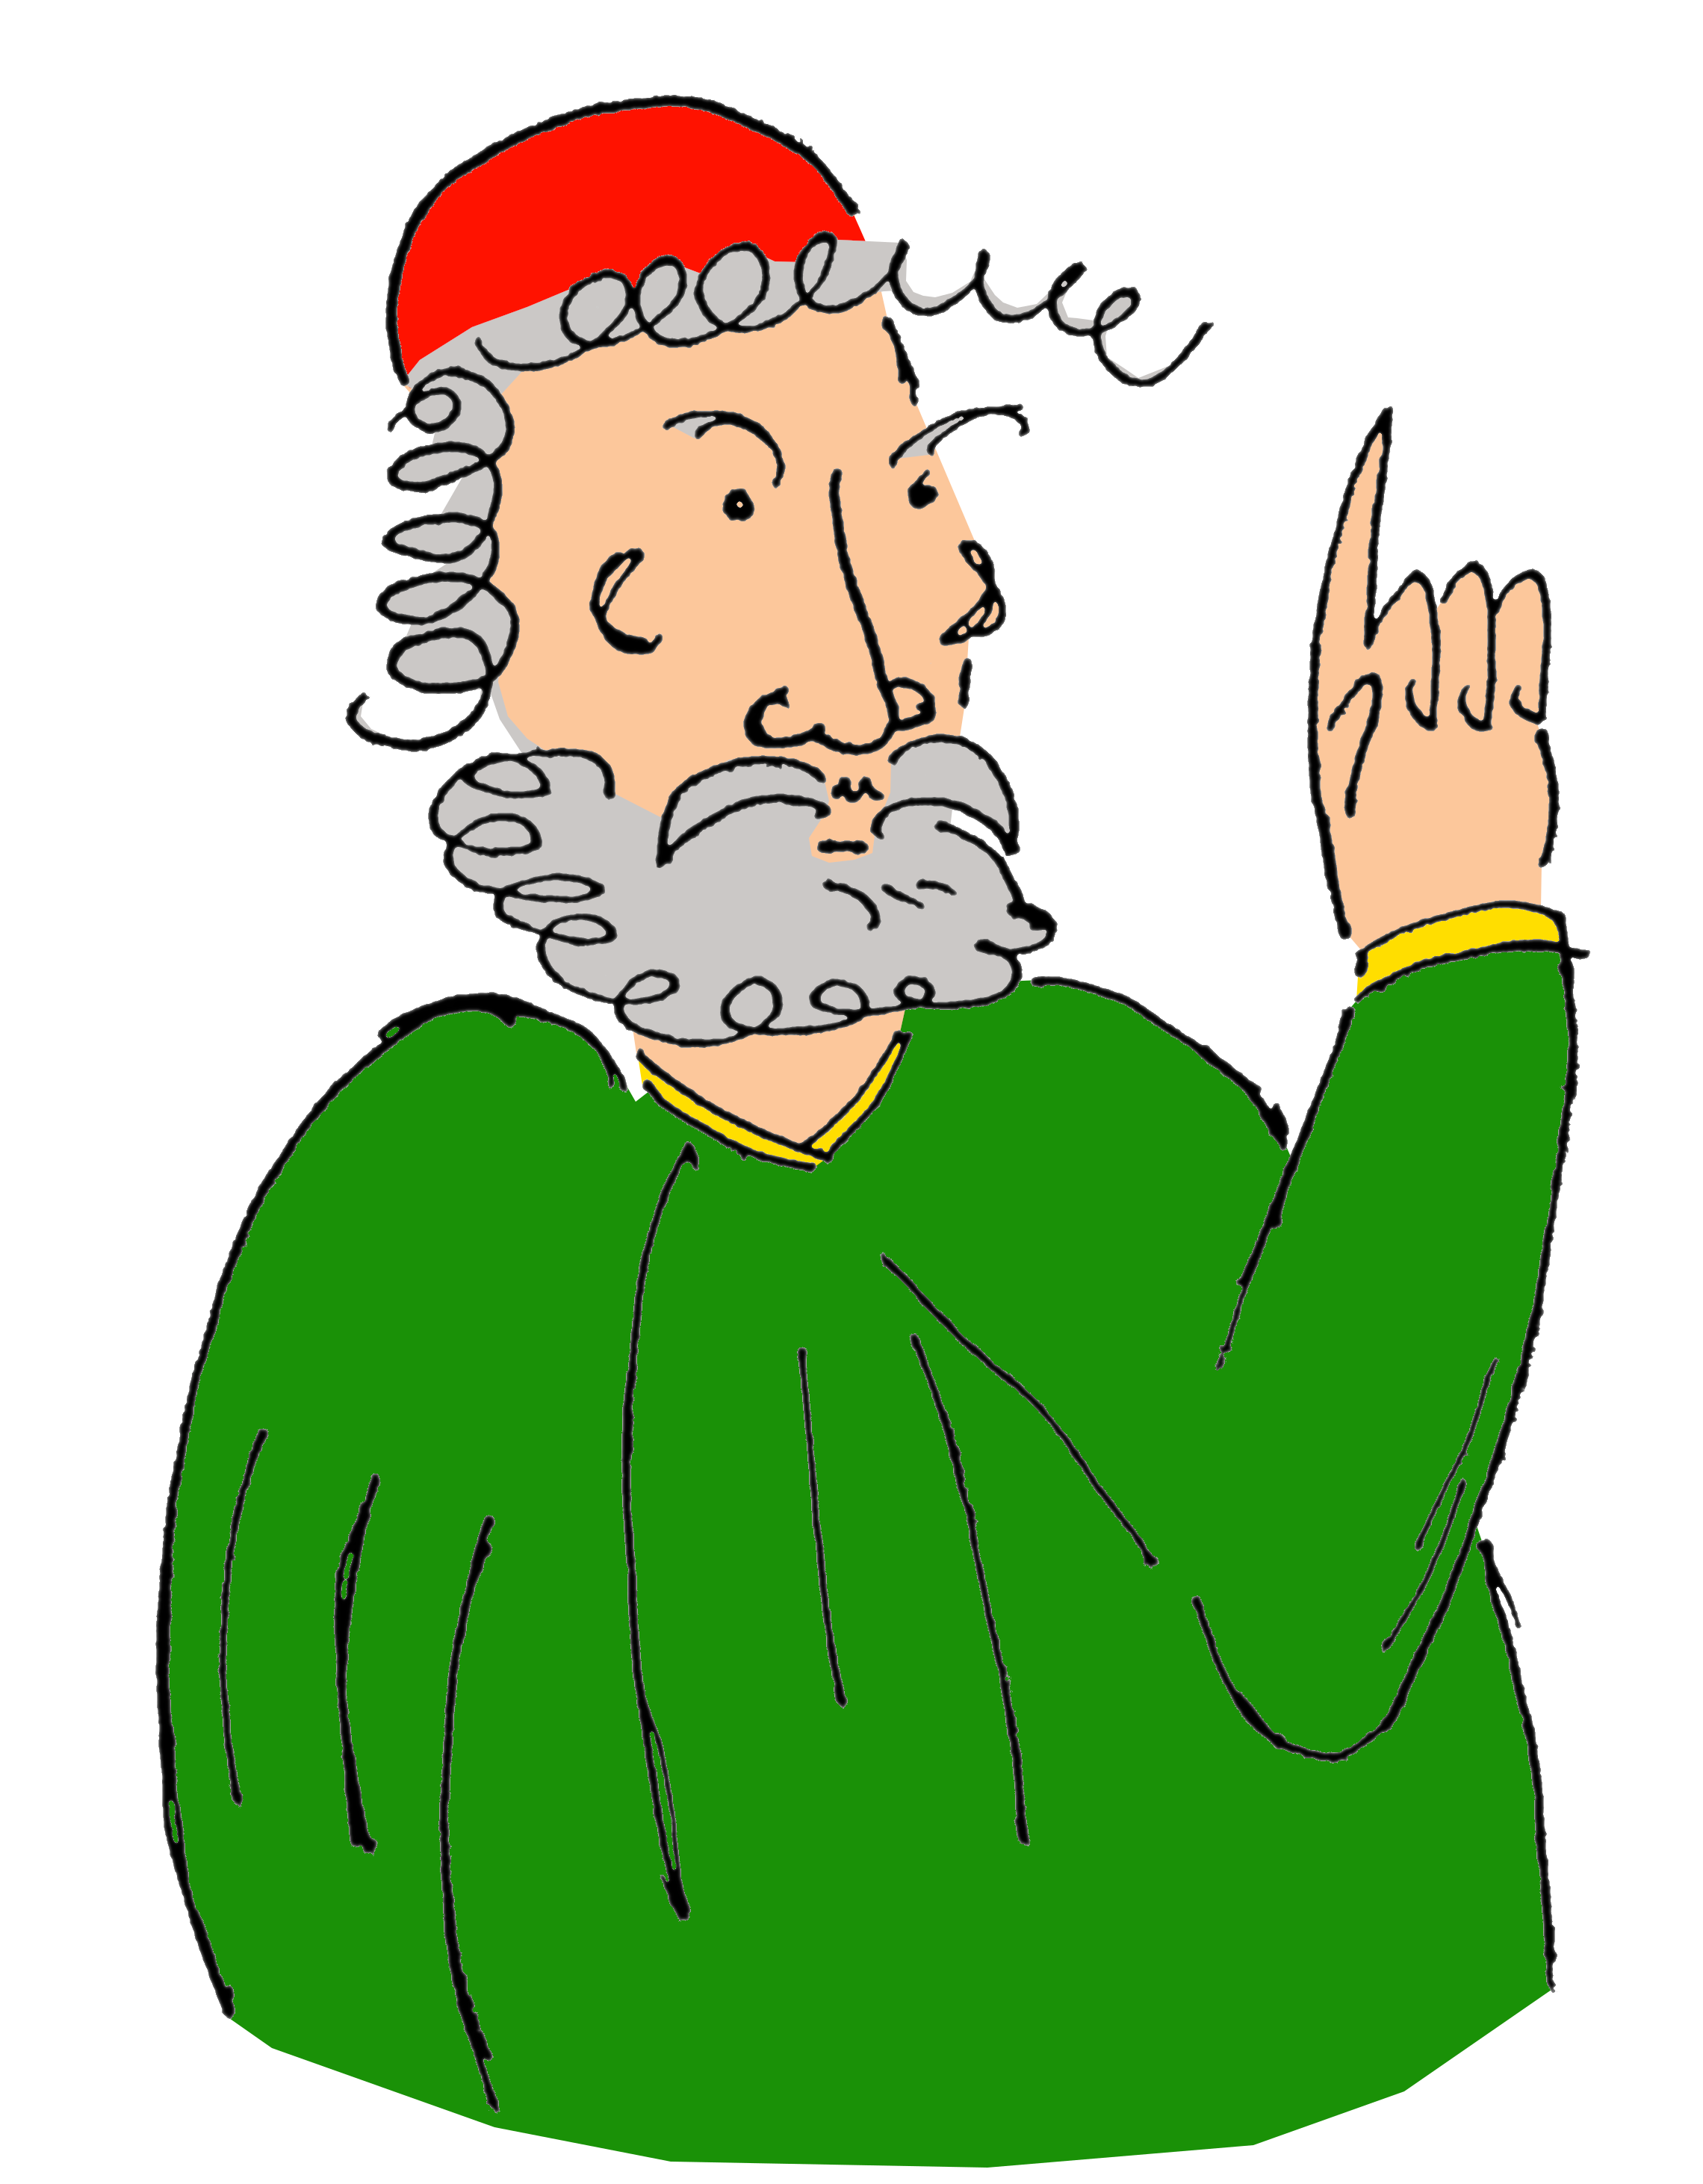
\includegraphics[width=8cm]{tolomeo}};
			\node (example-textwidth-2) [notice={(-3,-1)}, ultra thick, right, align=center, text width=12cm, color=black, fill=white, font=\fontsize{23pt}{24pt}\selectfont] at (8,4.5) {Signora maestra! La Luna fa i dispetti al Sole!};
			\node (example-textwidth-2) [notice={(3,1)}, ultra thick, right, align=center, text width=12cm, color=black, fill=white, font=\fontsize{23pt}{24pt}\selectfont] at (8,-4) {Tolomeo! Stai attento alla lezione! Non guardare le stelle!};
		\end{scope}
		%dida
		\begin{scope}[shift={(0,-29)}]
			\draw [ultra thick, fill=dida] (1,3) rectangle (29,-3);
			\node (example-textwidth-2) [right, align=left, text width=27cm, color=black, font=\fontsize{23pt}{24pt}\selectfont] at (1.5,0) {Tolomeo, in realtà, le stelle le ha guardate. E alla fine ha redatto un catalogo con 48 costellazioni. E non si è fermato qui: ha proposto un modello per descrivere il moto dei corpi celesti e ha descritto il fenomeno di cui ci occupiamo oggi, l'eclissi di Sole.};
		\end{scope}
		%eclipse
		\begin{scope}[shift={(0,-37.5)}]
			\draw [ultra thick, fill=space] (1.5,4.5) rectangle (28.5,-52);
			%dida
			\draw [ultra thick, fill=dida] (16.5,3.5) rectangle (29,-3.5);
			\node (example-textwidth-2) [right, align=left, text width=11.5cm, color=black, font=\fontsize{23pt}{24pt}\selectfont] at (17,0) {L'eclissi di Sole è un fenomeno astronomico che accade quando la Luna si trova a passare tra la Terra e il Sole.\\Esistono vari tipi di eclissi solari.};
			%dida
			\begin{scope}[shift={(0,-8.5)}]
				\draw [ultra thick, fill=dida] (16.5,3.5) rectangle (29,-2);
				\node (example-textwidth-2) [right, align=left, text width=11.5cm, color=black, font=\fontsize{23pt}{24pt}\selectfont] at (17,1) {\textbf{Eclissi totale}: quando la Luna oscura completamente il Sole.\\Si osserva nelle zone del cono d'ombra.};
			\end{scope}
			%dida
			\begin{scope}[shift={(0,-15.5)}]
				\draw [ultra thick, fill=dida] (16.5,4) rectangle (29,-2);
				\node (example-textwidth-2) [right, align=left, text width=11.5cm, color=black, font=\fontsize{23pt}{24pt}\selectfont] at (17,0.9) {\textbf{Eclissi parziale}: quando la Luna non riesce a oscurare completamente il Sole a causa di un non perfetto allineamento. Si osserva nelle zone di penombra.};
			\end{scope}
			% sun
			\tkzDefPoint(11,-2){A}
			\tkzDefPoint(17,-2){B}
			\tkzDefCircle[radius](A,B)
			% moon
			\tkzDefPoint(11,-20){L}
			\tkzDefPoint(13,-20){C}
			\tkzDefCircle[radius](L,C)
			% earth
			\tkzDefPoint(11,-39.5){E}
			\tkzDefPoint(11,-29){D}
			\tkzDefCircle[radius](E,D)
			%
			\tkzTangent[from=D](L,C) \tkzGetPoints{d}{e}
			%
			\tkzInterLC(D,e)(A,B) \tkzGetPoints{s1}{s2}
			\tkzInterLC(D,d)(A,B) \tkzGetPoints{s3}{s4}
			%
			\tkzTangent[from=s1](E,D) \tkzGetPoints{l1}{l2}
			\tkzTangent[from=s4](E,D) \tkzGetPoints{l3}{l4}
			%
			\tkzInterLL(D,s1)(s4,l3) \tkzGetPoint{c1}
			\tkzInterLL(D,s4)(s1,l2) \tkzGetPoint{c2}
			\tkzInterLL(s1,l2)(s4,l3) \tkzGetPoint{c3}
			%
			\tkzDrawPolygon[fill=white,opacity=0.5](s1,s4,c2,c1)
			\tkzDrawPolygon[fill=white,opacity=0.5](s1,s4,c3)
			\tkzDrawPolygon[fill=white,opacity=0.5](c3,c2,c1)
			\tkzDrawCircle[fill=moon](L,C)
			\tkzDrawCircle[fill=earth](E,D)
			\tkzDrawPolygon[fill=craterm,opacity=0.4](c1,c2,l2,l3)
			\tkzDrawPolygon[fill=craterm,opacity=0.6](c1,c2,D)
			\tkzDrawCircle[fill=white](A,B)
			%
			\tkzDefPoint(11,-25.5){O}
			\tkzDefPoint(5,-20){d1}
			\tkzDrawVectors[color=white, ultra thick](d1,O)
			\node (example-textwidth-2) [right, align=left, text width=11.5cm, color=white, font=\fontsize{18pt}{19pt}\selectfont] at (2,-19.5) {Cono d'ombra};
			%dida
			\begin{scope}[shift={(0,-23)}]
				\draw [ultra thick, fill=dida] (16.5,3.5) rectangle (29,-16);
				\node (example-textwidth-2) [right, align=left, text width=11.5cm, color=black, font=\fontsize{23pt}{24pt}\selectfont] at (17,0.9) {\textbf{Eclissi anulare}: quando la dimensione apparente della Luna è più piccola del disco solare:};
				\draw [fill=white] (23,-7) circle (5cm);
				\draw [fill=black] (23,-7) circle (4.5cm);
				\node (example-textwidth-2) [right, align=left, text width=11.5cm, color=black, font=\fontsize{23pt}{24pt}\selectfont] at (17,-14) {In questo caso si osserva un disco nero circondato da un anello di luce.};
			\end{scope}
			%
			\tkzDefPoint(13,-25.5){P}
			\tkzDefPoint(17,-19){d2}
			\tkzDrawVectors[color=white, ultra thick](d2,P)
			\node (example-textwidth-2) [right, align=left, text width=11.5cm, color=white, font=\fontsize{18pt}{19pt}\selectfont] at (17,-18.5) {Penombra};
			%dida
			\begin{scope}[shift={(0,-44)}]
				\draw [ultra thick, fill=dida] (16.5,3.5) rectangle (29,-2);
				\node (example-textwidth-2) [right, align=left, text width=11.5cm, color=black, font=\fontsize{23pt}{24pt}\selectfont] at (17,0.9) {\textbf{Eclissi ibrida}: in alcune zone della Terra appare come un'eclissi totale, in altre come eclissi anulare. E' molto rara.};
			\end{scope}
		\end{scope}
		%
		\begin{scope}[shift={(0,-92.5)}]
			\draw [ultra thick, fill=dida] (1.5,2.5) rectangle (28.5,-2.5);
			\node (example-textwidth-2) [right, align=left, text width=25.5cm, color=black, font=\fontsize{23pt}{24pt}\selectfont] at (2,0) {Dal punto di vista geometrico, l'eclissi solare è possibile poiché le dimensioni apparenti del disco lunare coincidono con le dimensioni apparenti del disco solare. Ricordiamo, infatti che il Sole ha un raggio medio di poco meno di $7 \cdot 10^{8} m$, mentre la Luna di $1.7 \cdot 10^{6} m$.};
		\end{scope}
		%
		\begin{scope}[shift={(0,-98)}]
			\draw [ultra thick, fill=space] (1.5,2.5) rectangle (28.5,-35);
			% sun
			\tkzDefPoint(10,-27){S}
			\tkzDefPoint(10,-21){R3}
			\tkzDefCircle[radius](S,R3)
			% moon
			\tkzDefPoint(18.5,-8){L}
			\tkzDefPoint(18.5,-9){R2}
			\tkzDefCircle[radius](L,R2)
			% earth
			\tkzDefPoint(21,-3.5){E}
			\tkzDefPoint(21,-7.5){R1}
			\tkzDefCircle[radius](E,R1)
			%
			\tkzDefPoint(19,-5){O1}
			\tkzTangent[from=O1](S,R3) \tkzGetPoints{s1}{s2}
			\tkzTangent[from=s1](L,R2) \tkzGetPoints{la}{lb}
			\tkzTangent[from=s2](L,R2) \tkzGetPoints{lc}{ld}
			%
			\tkzInterLL(s1,lb)(s2,lc) \tkzGetPoint{Eo}
			%
			\tkzDrawArc[rotate,color=earth,thick](S,E)(40)
			\tkzDrawArc[rotate,color=earth,thick](S,E)(-18)
			\begin{scope}[yscale={0.4}]				
				\tkzDrawArc[rotate,color=moon,thick](E,L)(50)
				\tkzDrawArc[rotate,color=moon,thick](E,L)(-205)
			\end{scope}			
			%
			\tkzDrawCircle[fill=earth](E,R1)
			\tkzDrawCircle[fill=moon](L,R2)
			\tkzDrawCircle[fill=white](S,R3)
			\tkzDrawCircle[R,fill=craterm, opacity=0.5](Eo, 2.4cm)
			\tkzDrawCircle[R,fill=black](Eo, 0.2cm)
			%
			\tkzDrawSegments[color=black](s1,Eo)
			\tkzDrawSegments[color=black](s2,Eo)
			\tkzDrawLines[color=black,add = 0 and 0.2](s1,la)
			\tkzDrawSegments[color=black,add = 0 and 0.2](s2,ld)
		\end{scope}
		%
		\begin{scope}[shift={(0,-138.5)}]
			\tkzDefPoint(28,0){H}
			\tkzDefPoint(21,3){M}
			\tkzDefPoint(22.5,3){Mr}
			\pic at (H) {human};
			\tkzDrawCircle[fill=moon](M,Mr)
			\tkzTangent[from=H](M,Mr) \tkzGetPoints{m1}{m2}
			\tkzCalcLength[cm](H,m1)  \tkzGetLength{dArc}
			\tkzDrawSegments[color=black](H,m1 H,m2)
			\tkzDrawArc[R,arc,color=space](H,1/3*\dArc)(140,172)
			%
			\tkzDefPoint(25.5,0.5){V1}
			\tkzDefPoint(22.5,-1.5){V2}
			\tkzDrawVectors[color=black, ultra thick](V2,V1)
			\node (example-textwidth-2) [right, align=left, text width=6cm, color=black, font=\fontsize{15pt}{16pt}\selectfont] at (20.5,-3) {Le dimensioni apparenti della Luna sono anche dette diametro angolare};
			%
			\draw [ultra thick, fill=dida] (1.5,5) rectangle (18.5,-5);
			\node (example-textwidth-2) [right, align=left, text width=16cm, color=black, font=\fontsize{23pt}{24pt}\selectfont] at (2,0) {Sempre dal punto di vista geometrico, l'eclissi anulare è spiegabile ricordando che l'orbita della Luna intorno alla Terra è leggermente ellittica, quindi le dimensioni apparenti della Luna risultano variabili. In particolare durante le eclissi anulari la Luna è più lontana, quindi il suo disco appare più piccolo.};
		\end{scope}
		%
		\begin{scope}[shift={(0,-144.5)}]
			\node at (27,0) () {
\includegraphics[width=3.7cm]{licenza}};
			\node at (18,-0.1) {\textcolor{black}{\fontsize{14}{15}\selectfont Testo e illustrazioni: @ulaulaman - Gianluigi Filippelli}};
		\end{scope}
	\end{tikzpicture}
%
\end{document}